\documentclass[10pt,a4paper]{book}
\usepackage[utf8]{inputenc}
\usepackage[portuguese]{babel}
\usepackage[T1]{fontenc}
\usepackage{amsmath}
\usepackage{amsfonts}
\usepackage{amssymb}
\usepackage{listings}
\usepackage{imakeidx}
\usepackage{graphicx}
\usepackage{lmodern}
\usepackage[left=2cm,right=2cm,top=2cm,bottom=2cm]{geometry}
\author{Duarte Ferreira Dias }
\title{Sebenta AC1}
 \makeindex

\begin{document}
\maketitle
\tableofcontents{}
\chapter{Disclaimer}

	Esta sebenta tem como objetivo principal ajudar todos os deseperados em fazer AC1 com o mínimo de esforço possível,(ou pelo menos com a menor dispersão possível :-).

	Os conteúdos são baseados nos slides disponibilizados no e-learning e no livro recomendado pela regência da cadeira(Henessey).

	A leitura deste texto de apoio(Sebenta) não dispensa a ida às aulas (Excepto se forem as do Ferrari(aka:Fiat Panda) eheh, se a regência for outra, os professores são excelentes e esforçam-se por tornar a matéria acessível tal como esta sebenta pretende) nem adispensa a leitura quer do livro quer dos slides.

	Para quem quiser experimentar o mundo do latex está livre de adicionar conteúdo e adicionar o se nome como co-autor da sebenta.

	Boa Sorte e Votos de Bom Estudo

	#eetésolidário #odetienosso

	PS: tb já há uma sebenta de AC2 :-)

%!TeX spellcheck = pt-PT

\chapter{Estrutura básica de um Processador}

	Os cinco componentes básicos de um computador são o input, output, memória, \textit{datapath} e controlo.Estando os últimos dois elementos, geralmente integrados no processador.

	Segundo o modelo de von Neumann existem três tipos de BUS.
		\begin{itemize}
			\item \textbf{Data Bus}: barramento de transferência de informação;
			\item \textbf{Adress Bus} : identifica a origem/destino da informação;
			\item \textbf{Control Bus} : sinais de protocol especificam o modo como a transferência deve ser feita;
		\end{itemize}

 \chapter{Operações na Arquitectura MIPS}

	\section{Operações Ariteméticas}

	  Na arquitectura MIPS existem várias instruções aritméticas das quais se destacam :
	    \begin{enumerate}
	     \item add rd,rs,rt: corresponde à adição de b a c cujo resultado é guradado em \$rd;
	     \item addu rd,rs,rt adição de grandezas sem sinal;
	     \item sub rd,rs,rt : subtração de b a c armazenada em \$rd;
	     \item subu rd,rs,rt;
	    \end{enumerate}

	    \subsection{Adição e Subtração}
	    	Na Arqutectura MIPS a adição é feita bit a bit da direita para a esquerda somando o carry se necessário. A subtração assenta na adição pelo que o um dos operandos é negado.

	    	O overflow da operação ocorre quando o valor calculado excede o limite da representação.

	    	Abaixo estão representadas as condições para as quais existem overflow na soma e subtração.


			\begin{figure}[htp]
			    \centering
			    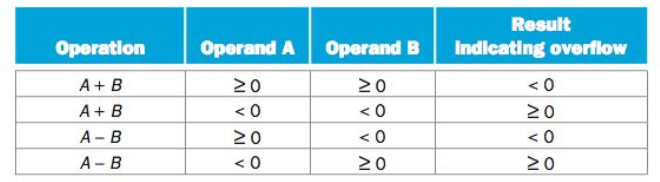
\includegraphics[scale=0.4]{of.png}
			    \caption{Condições que comfirmam a existência de Overflow}
			    \label{OF}
			\end{figure}

			As instruções add,addi e sub originam uma excepção no sistema quando é detetado overflow na operação.

			Já as instruções addu,addiu e subu não lançam essas excepções.

			Uma vez que a linguagem C ignora as situações de overflow, por isso os compiladores C do MIPS e geram sempre as versões sem sinal das operações ariteméticas(unsigned).

	    \subsection{Exemplo 1}
	     Vamos efectuar as operações add e sub.
	      \begin{lstlisting}
		f = (g+h)-(i+j); // Sintaxe em C
	      \end{lstlisting}

	     \begin{lstlisting}
		#Sintaxe em Assembly do MIPS
		add $t0,$1,$2;  # $t0 contem $1 e $2 -> g+h
		add $t1,$3,$4;  # $t1 contem $3 e $4 -> i+j
		sub $s0,$t0,$t1;

	     \end{lstlisting}

	     \subsection{Mutlipicação}

	     Usando as operações mult e mulu é possivel multiplicar o conteudo de dois registos

	     Numa primeira abordagem a execução desta operação consite em replicar em hardware as iterações que se fazem no papel.

   			\begin{figure}[htp]
			    \centering
			    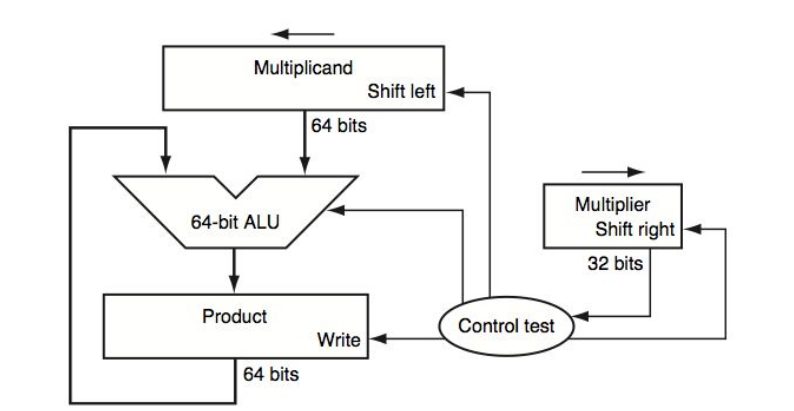
\includegraphics[scale=0.5]{mul1.png}
			    \caption{Primeira Implementação de um muiltiplicador}
			    \label{mul1}
			\end{figure}

		Seguindo o método usual seria necessário shiftar 32 vezes o multiplicando para efetuar a operação. Essa operação de shift implica que o multiplicando se mova 32 bits para a esquerda, obrigndo a que o registo que o alberga tenha 64 bits de tamanho.Esse registo é shiftado um bit para a esquerda por cada iteração.

		Os três passos de execução apresentados são repetidos 32 vezes para executar a multiplicação.Se cada operação fosse feita a cada ciclo de relógio demoraria 96 ciclos de relógio a se executada, o que torna a implementação bastante ineficiente.

		Uma forma de otimizar este processo é paralelizar algumas das operações, reduzindo significativamente os ciclos de relógio, mais especificamente $1/3$ dos ciclos necessários.Podemos com esta configuração efetuar a operação com uma iteração por ciclo de relógio.

		Outra maneira utilizada pelos compiladores do MIPS é usar shifts para a esquerda ao invés da multiplicar, porém só é valido quando os registos são multiplicados por constantes, ou registos cujo valor equivalha a uma potência de dois;

   			\begin{figure}[htp]
			    \centering
			    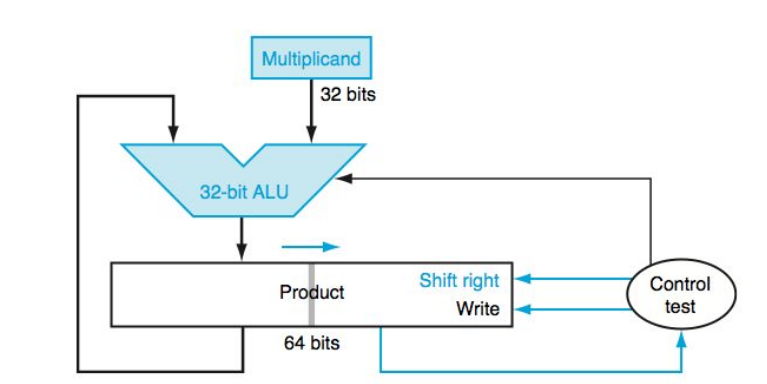
\includegraphics[scale=0.5]{mul2.png}
			    \caption{Implementação otimizada de um multiplicador}
			    \label{mul2}
			\end{figure}

		Resta abordar a forma como se armazena o resultado da operação uma vez que o tamanho do produto é de 64 bits.O MIPS disponibiliza dois registos de 32 bits para armazenar o produto um chama-se Hi e o outro Lo. Para buscar o valor na forma de inteiro de 32 bits é usada a pseudoinstrução mflo(\textit{move from lo}).




	\section{Operaçõe s Load Store}

	  Como as operações ariteméticas operam apenas sobre registos, torna-se necessária  a criação de instruções que permitam carregar(\textit{load}) e guardar(\textit{store}) os valores dos registos da e para a memória.
	  Surge, então, duas operações, a \textit{load-word} com a sintaxe \textbf{lw}\$rd,offset(\$registobase) e que permite a transferência de dados da memória para um regsto de destino, já a instrução \textit{load-word}  \textbf{sw}\$rs,offset(\$registobase) 	  que por oposição guarda na memória os valores de um registo.

	   \subsection{Exemplo 2}
	      Aplcação da instrução \textit{load-word}

	      \begin{lstlisting}
		//sintaxe C
	        g = h + A[8];

	        #sintaxe Assembly do MIPS
	        lw $t0,32($s3);   #offset (4*8) da memoria
	        add %s1;$s2,$t0; #soma
	      \end{lstlisting}

	      Outro Exemplo agora com a aplicação de ambas as operações.

	     \begin{lstlisting}
		//sintaxe C
	        A[12] = h + A[8];

	        #sintaxe Assembly do MIPS
	        lw $t0,32($s3);   #leitura com offset (4*8) da memoria
	        add %s1;$s2,$t0;  #soma
	        sw $s2,48($s4);	  #armazenamento com offset (12*4) da memoria
	      \end{lstlisting}

	  \section {Operações com constantes e imediatos}

	      Grande parte dos programas recorre a um numero de variáveis maior que o o número de registos do processador. Por isso o compilador tenta guardar apenas aquelas variáveis que
	      que são mais utilizadas nos registos e move as outras para a menmória.

	      Um dos principios fundamentais do design de processadores surgere que a velocidade de acesso aos registos é maior que a de acesso à memória.

	      Para implementar operações com imediatos pode-se recorrer ás seguintes instruções:

		\begin{lstlisting}
		  lw $t0,const4addr($s1);#t0 = 4
		  add $s3,$s3,$t0; #s3 = s3 + t0(4)
		\end{lstlisting}

	      A alternativa para implementar esta instrução é usar:

		\begin{lstlisting}
		  addi $s3,$s3,4;
		\end{lstlisting}

	      O MIPS aceita nativamente esta instrução, permitiundo suprimir o uso da instrução lw juntamente com a add, optimizando assim a execução do programa.

	  \section{Operações Lógicas}

	    O mips suporta as seguintes operações lógicas:
	      \begin{itemize}
	       \item sll -> shift left logical;
	       \item srl-> shift right logical;
	       \item and,andi -> bitwise AND(pode ser feito com um imediato);
	       \item or,ori   -> bitwise OR (pode ser feito com um imediato);
	       \item nor;
	      \end{itemize}

	      Uma aplicação bastante não tão óbvia do shift left logical permite multiplicar o valor do registo a shiftar pela potencia de 2 da quantidade de shift.

	    \subsection{Exemplo 3}

	      A operação de shift left logical :

	      \begin{lstlisting}
		sll $t2,$t0,4 # $t2 = $t0 <<4;
	      \end{lstlisting}

	      \begin{center}
\begin{tabular}{|l|l|l|l|l|l|}\hline
op & rs & rt & rd & shmnt & funct\\\hline
0 & 0 & 16 & 10 & 4 & 0\\\hline
	      \end{tabular}
	      \end{center}


  \section{Operações de Salto Condicional}

  As estruturas de decisão mais usadas em programação são os if's. As instruções que permitem implementar essas estruturas em MIPS são:
    \begin{itemize}
     \item beq \$rd,\$rt,label -> branch if equal -> consiste em comparar valores de dois registos e deteminar se são iguais;
     \item bne \$rd,\$rt,label-> branch not equal -> consiste em determinar se dois registos são diferentes slatando para uma label onde estará o conjunto de instruções que deve ser executado caso a instrução se confirme.
    \end{itemize}

     \subsection{Nota sobre as operações virtuais}

	Todas as outras operações de salto condicional resultam da conjugação da operação (slt ou slti) que retorna um caso o valor lógico 1 caso o primeiro registo seja menor do que o o segundo e 0 caso o contrário.

	A conjugação do set on less com as operações de salto condicional bne e beq permitem impelemtar as operações:
	    \begin{itemize}
	     \item bge;
	     \item bgt;
	     \item ble;
	     \item bnez;
	     \item beqz;
	     \item blt
	   \end{itemize}

 	\section{Operações de salto}

 		Estas operações são necessárias para efetuar um salto de uma instrução para a outra.

 		Existem três operações de salto a JAL , JR e J.

 		A jal (mais conhecida por \textit{jump and link}) é utilizada para saltar para o endereço da instrução que cooresponde ao inicio duma função, para elem disso guarda o valor do Program Counter e adiciona-he mais quatro para que quando a função acabar de executar e retornar o resultado ela vai saltar para o endereço da instrução seguinte à da execução da função;

 		O jr ou  \textit{Jump Register}  consiste em saltar para um endereço especificado por um registo.




 \chapter{Memória do MIPS}
    Todas as linguagens de programação suportam vários tipos de dados cuja complexidade pode variar do muito simples(constantes, variáveis) para tipos de dados mais complicados(são exemplo os arrays e estruturas de dados).
    Uma vez que o processador não consegue armazenar grandes volumes de dados no seu interior( 32 registos de 32 bits no caso do MIPS), este delega essa função para a memória que por sua vez é capaz de guardar grandes volumes de dados.

    Por vezes torna-se útil endereçar individualmente cada um dos quatro bytes que constitui uma palavra. Pode-se dizer que a memória é\textit{byte-adressable}
    É por isso que na arquitetura MIPS o endereçamento à memória deve ser feito em múltiplos de quatro.
    Para que este tipo de endereçamento seja possível é necessário inserir um offset para aceder aos vários bytes que constituem a palavra.
    Este método de endereçar os dados armazenados permite otimizar a performance geral do sistema pois otimiza as transferências na memória.


 \chapter{ISA-Instruction Set Architecture}

	De uma forma geral, o CPU segue a seguinte ordem de execução das instruções que lhe são fornecidas:
		\begin{enumerate}
			\item \textbf{Instruction Fetch} -> passo no qual é feita a leitura de código máquina da instrução.(Instrução reside em memória);
			\item \textbf{Instruction Decode} -> nesta fase é feita a descodificação da instrução pela unidade de controlo presente no processador;
			\item \textbf{Operand Fetch} -> leitura dos operandos;
			\item \textbf{Execute} -> é feita a execução da operação especificada pela instrução;
			\item \textbf{Store Result} -> o resultado das operações efetuadas no passo anterior são posteriormente transferidas para o o registo especificado pela operação.
		\end{enumerate}

	O \textit{Instruction Set} propriamente dito corresponde ao conjunto de instruções que o processador é capaz de executar.
	Por norma cada arquitetura de processadores ou micro-controladores tem o seu \textbf{Instruction Set} dentro das mais populares destacam-se os ISA's do MIPS, ARM, Intel x86, Power PC e Cell;


	\section{Instruções}

	Na arquitetura MIPS existem três tipos de instruções.Estas instruções servem têm comportamentos diferentes assim como fins diferentes.

	Todas as instruções do MIPS são armazenadas em registos de 32 bits tendo o tamanho fixo.

	O número de registos disponíveis é de 32 bits.Este número reduzido de registos deve-se principalmente a duas razões. Uma delas é que ao aumentar o número de registos aumenta-se o número de
	ciclos de relógio necessários para o acesso à memória, reduzindo a performance do processador, a outra prende-se com manter o tamanho das instruções pois aumentando o numero de registos era necessário
	aumentar a quantidade de bits nos campos de endereçamento da memória.

	\subsection{Instruções do tipo R}

	Estas instruções são responsáveis pelas operações lógicas e aritméticas.

	Têm como operandos os seguintes elementos:
	 \begin{itemize}
	 	\item \textbf{op} : mais conhecido por opcode, representa a operação da instrução que foi dada-6 bits;
	 	\item \textbf{rs} : o operando do segundo registo-5 bits;
	 	\item \textbf{rt} : operando do segundo registo-5 bits;
	 	\item \textbf{rd} : registo de destino onde é guardado o resultado da operação a executar-5bits.
	 \end{itemize}


	\begin{figure}[htp]
	    \centering
	    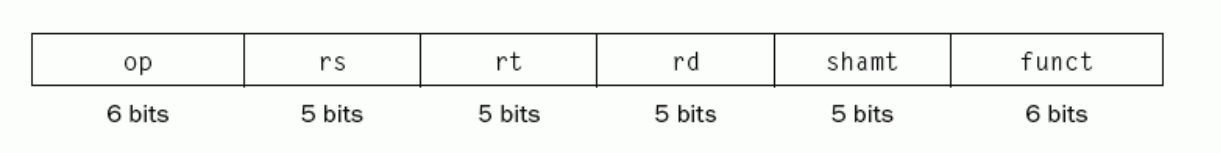
\includegraphics[scale=0.4]{fig1.png}
	    \caption{configuração das intruções do tipo R}
	    \label{insturçãor}
	\end{figure}



	\subsection{Instruções do tipo I}

	As instruções do tipo I são usadas para exprimir as operações de leitrua e escrita na memória assim como as operações com imediatos.

	Por permitir o endereçamento à memoria e representação de constantes a configuração das istruções é diferente.
	É de notar que a arquitetutra MIPS opta por manter o tamanho das intruções fixo (32 bits) alterando-se o tamanho de alguns dos campos da instrução..

	Têm como operandos os seguintes elementos:
	 \begin{itemize}
	 	\item \textbf{op} : mais conhecido por opcode, representa a operação da instrução que foi dada-6 bits;
	 	\item \textbf{rs} : registo sobre o qual vais ser processada a operação-5 bits;
	 	\item \textbf{rt} : opernado que armazena o registo com o valor base do endereçamento-5 bits;
	 	\item \textbf{offset} : registo no qual é armazenado o endereço da memória ou o valor da constante a ser carregado-16bits;
	 \end{itemize}

	\begin{figure}[htp]
	    \centering
	    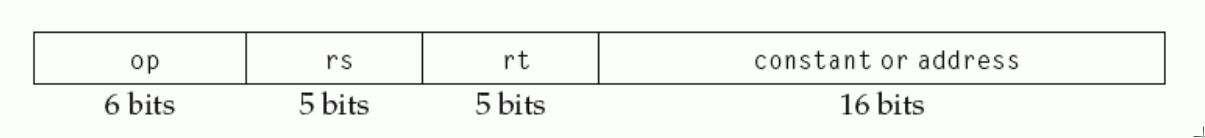
\includegraphics[scale=0.4]{instI.png}
	    \caption{configuração das intruções do tipo I}
	    \label{insturçãoi}
	\end{figure}

	  \subsection*{Exemplo 1}

	  \begin{lstlisting}
	    lw $t0,32($s3)  #$s3 => 19
	  \end{lstlisting}

	  Ao utilizar esta operção iriamos obter uma istrução do tipo I com os seguintes valores nos seus campos:


	  {%
\newcommand{\mc}[3]{\multicolumn{#1}{#2}{#3}}
\begin{center}
\begin{tabular}{|llll|}\hline
\mc{1}{|l|}{opcode} & \mc{1}{l|}{rs} & \mc{1}{l|}{rt} & offset\\\hline
\mc{1}{|l|}{35} & \mc{1}{l|}{19} & \mc{1}{l|}{8} & 32\\\hline

	  \end{tabular}
	  \end{center}
}%

 Ficamos com a seguinte instrução em binário 100011100111000000000000010000

	  \subsection{Exemplo 2}


	  \begin{lstlisting}

	   A[300] = h + A[300];//sintaxe em c

	   lw $t0,1200($t1)
	   add $t0,$t0,$s2
	   sw $t0,1200($t1)
	  \end{lstlisting}


\newcommand{\mc}[3]{\multicolumn{#1}{#2}{#3}}
\begin{center}
\begin{tabular}{|llll|}\hline
\mc{1}{|l|}{opcode} & \mc{1}{l|}{rs} & \mc{1}{l|}{rt} & offset\\\hline
\mc{1}{|l|}{35} & \mc{1}{l|}{19} & \mc{1}{l|}{8} & 1200\\\hline

	  \end{tabular}
	  \end{center}

%\newcommand{\mc}[3]{\multicolumn{#1}{#2}{#3}}
\begin{center}
\begin{tabular}{|llll|}\hline
\mc{1}{|l|}{opcode} & \mc{1}{l|}{rs} & \mc{1}{l|}{rt} & offset\\\hline
\mc{1}{|l|}{43} & \mc{1}{l|}{9} & \mc{1}{l|}{8} & 1200\\\hline

	  \end{tabular}
	  \end{center}





  \chapter{Funções}

  	Na Arquitectura MIPS as funções seguem  a seguinte sequência de execução:

  	\begin{enumerate}
  		\item Colocar os argumentos nos registos \$a0,\$a1,\$sa2,\$a3 (exceção será abordado abaixo);
  		\item Começar a execução da função, faz-se por via da instrução jal (\textit{"jump and link"}) que guarda o endereço da instrução seginte em \$ra;
  		\item Alocar memória para a execução do procedimento;
  		\item Executar a função;
  		\item Guardar o valor de retorno em \$v0 ou \$v1;
  		\item Finalmente usa-se a instrução de salto jr com o valor de \$ra(registo que guarda o ponto a retornar) para saltar para a instrução seguinte função chamadora estava antes de iniciar a função.
	\end{enumerate}

		Existem dois tipos de funções:
		 \begin{itemize}
		    \item Folha : todo o conjunto de subrotinas que não chama uma subrotina;
		    \item Não Folha : analogamente são aquelas funções que chamam funções dentro de si mesmas.
		 \end{itemize}

 		Em casos normais a ordem de processamento segue a ordem desses pontos, porém quando os
 		valores de return ou argumentos são mais do que os que estão convencionados torna-se
 		necessário proceder com alguma cautela.

 		Relembrando que a função não pode deixar resíduos da sua execução qualquer, os registos
 		da função chamadora que forem precisos guardar têm que ser repostos imediatamente após a
 		 execução da função e com o valor que tinham quando antes da função ser executada.

 		A estrutura de dados ideal para implementar o que acima foi descrito é uma stack(LIFO).
 		A stack precisa de um ponteiro(\$sp, \textit{Stack Pointer}) que referencie o endereço que foi alterado mais recentemente por forma a permitir que a funcção a executar saiba onde guardar os seus dados assim como permite restaurar os valores antigos.
 		Por cada dado que é acrescentado é necessário dar um incremento de uma palavra ao \textit{Stack Pointer}(4bytes).
 		Por convenção uma pilha enche do endereço mais alto para o mais pequeno.Por isso quando se adiciona conteudo à mesma é necessário decrementar o valor do ponteiro.


 		\begin{figure}[htp]
	    	\centering
	    	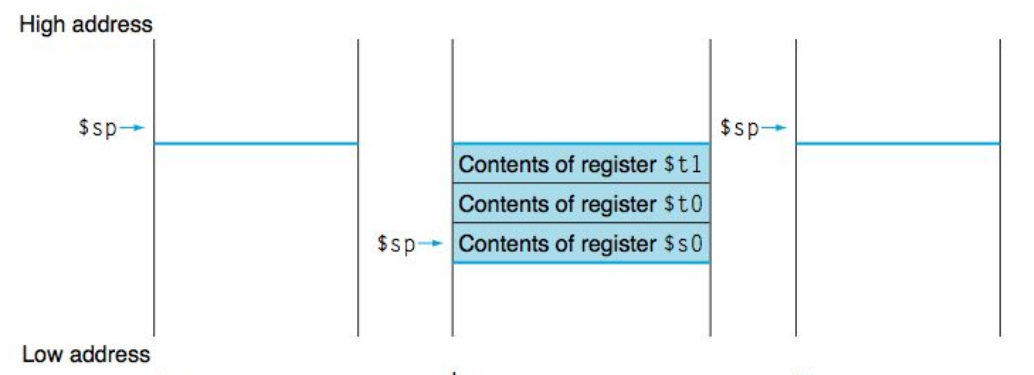
\includegraphics[scale=0.6]{stack1.png}
	    	\caption{Comportamento do \textit{Stack Pointer}}
	    	\label{stack 1}
		\end{figure}


 		\begin{figure}[htp]
	    	\centering
	    	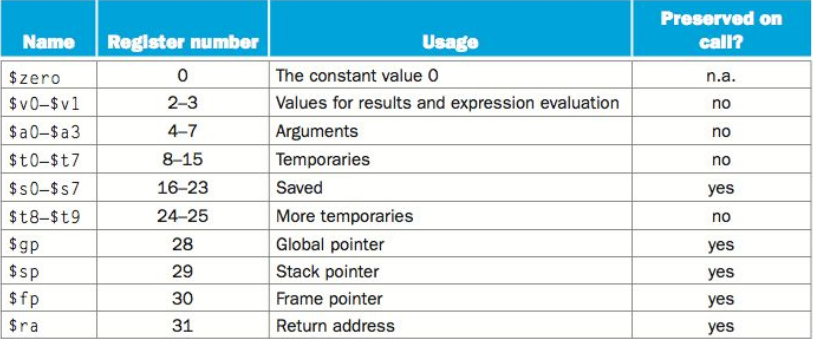
\includegraphics[scale=0.6]{registerconvention.png}
	    	\caption{Convenções dos Registos no MIPS}
	    	\label{conventions}
		\end{figure}

\chapter{Datapath}

		\section{Datapath Single Cycle}

			Nos capitulos acima forma descritas as instuções base do MIPS agora vamos tentar criar um processador que execute essas instruções o conjunto de blocos que as executa chama-se de datapath.

			Os dois primeiros passos de execução de uma instrução consistem em :

			\begin{enumerate}
				\item Usando o endereço de memória armazenado no PC para aceder à instrução armazenada na memória de instruções;
				\item Ler o conteudo de um ou dois registos(depende da instrução a executar);
			\end{enumerate}

			Depois destes dois passos iniciais dependendo do tipo de instrução a executar os dados vão seguir caminhos diferenntes.Dentro do mesmo tipo de instruções os elementos a usar não variam muito, tornando mais fácia a implementação do Datapath.

			Abaixo seguem os elementos base e as suas funcionalidades de um datapath single cycle.

			\paragraph{PC + Memória de Instruções}

				A junção do PC com a Memória de instruções e um adder permite-nos montar um circuito que permite efetuar o endereçamento à memória de instrução para poder dar inicio à execução de uma instrução o adder permite determinar qual o endereço da próxima instrução.Esse adder vai adicionar 4 bytes ao endereço atual do PC (PC+4).

			\paragraph{Registos}





		\section{Datapath Multi Cycle}

		    A implementação do datapath Multi Cycle consiste em dividir a execução de uma instrução em várias fases(operações).Cada uma dessas fases usa ium dos elemntos fundamentais(memória,register file ou ALU).
		    Em cada ciclo de relógio é possivel executar várias operações em paralelo desde que sejam independentes. Ao usar esta estratégia a frequêcia máxima de funcionamento depende apenas pelo maior dos tempos de atraso de cada um dos elementos.

		    A implementação deste datapath é feita com um máximo de 5 fases.

		    \subsection{Estrutura}

		    A versão multi-cycle do datapath em comparação ao datapath single-cycle terá apenas uma úncia memória (arquitectura \textit{Von Neumann}) e uma única ALU.

		    A existência de uma única memória implica que os acessos à memória de instrução e memória de dados sejam controlados para evitar que os dados na memória se corrompam.

		    Porque a execução de uma instrução vai demorar mais que um ciclo de relógio vai ser necessária a existência de registos à saída dos elementos funcionais para que, caso os valores produzidos pela unidade em causa sejam necessários no ciclo seguinte estes estejam resguardados. Foram então adicionados cinco registos, memória de dados, memória de instruções, A e B(encontram-se à saída do Register File) e ALUOut.

		    A utilização de apenas uma alu em comparação ao uso de uma alu mais dois somadores obriga a que se alterem o número de entradas dos multiplexer que se encontra à segunda entrada da ALU assim como adicionar um à primeira. Na primeira entrada o mux vai permitir selecionar a saída do registo A e a saída do Registo PC.No segundo mux é possível escolher entre o registo B a constante 4, o sinal proveniente do signal extender e por fim o sinal que vem do shift left 2.


		\begin{figure}[htp]
	    	\centering
	    	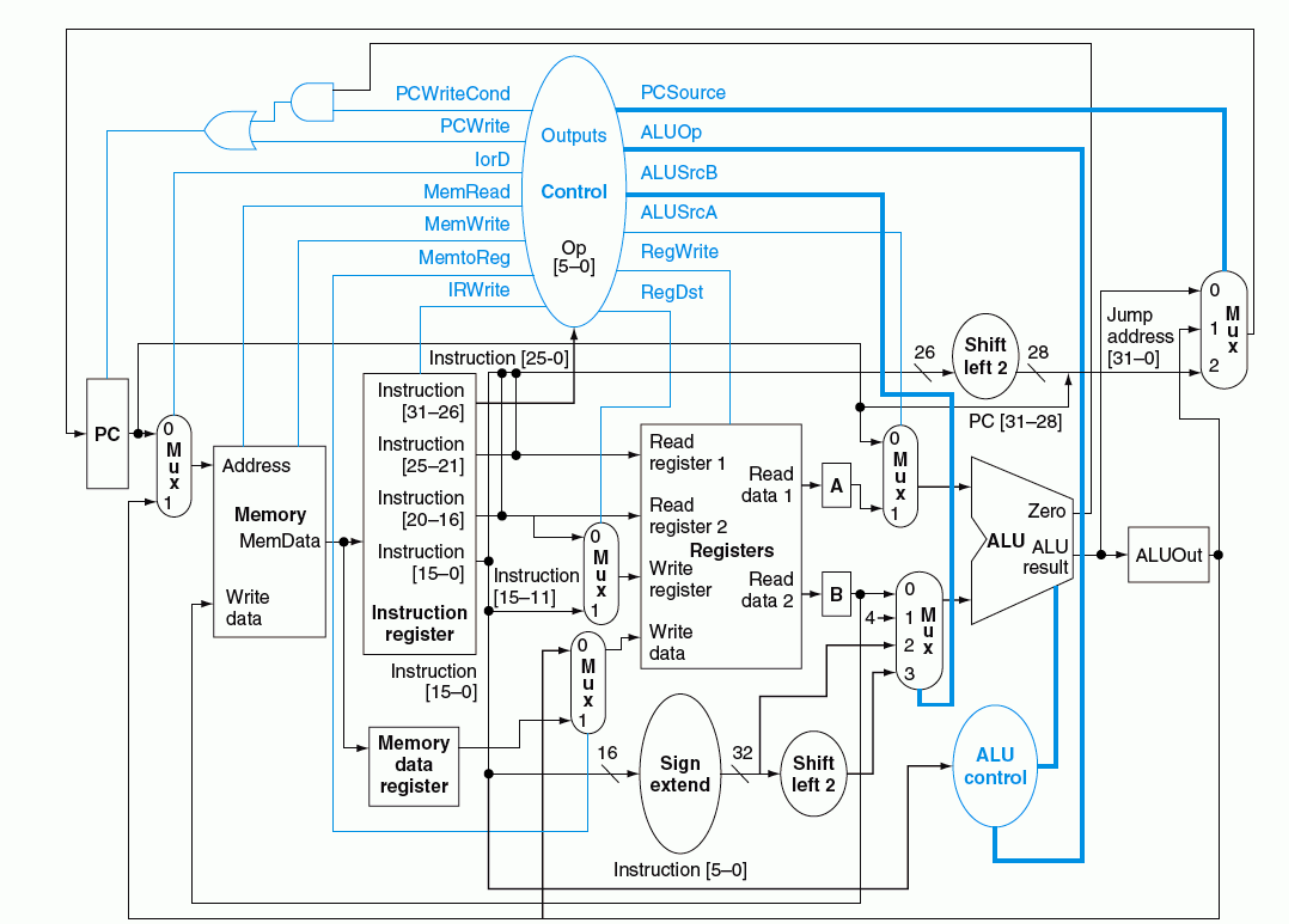
\includegraphics[scale=0.3]{mc1.png}
	    	\caption{Datapath multi-cycle completo}
	    	\label{multy-cycle Datapath}
		\end{figure}


		    \subsection{Fases de Execução}

		   O datapath abordado pela cadeira reconhece 5 fases de processamento. Sendo que as duas primeiras são comuns a qualquer instrução.A única instrução que faz uso das cinco fases de execução do MIPS é a instrução se LW, sendo que as operações de salto condicional(branch) e jump demoram apenas 3 fases(ou ciclos) e as instruções de escrita na memória(SW) e do tipo R demoram 4 fases(ou ciclos de relógio) a serem executadas.
		   Abaixo são descritas as operações executadas e os sinais de controlo usados em cada fase de execução mediante a instrução a executar.

			\subsubsection{Fase 1}

			É nesta fase que se efetua o instruction fetch(IF).

			É feita a escrita no instruction register através do endereçamento à memória(o PC é o endereço  usado) e o PC é incrementado por quatro(PC +4).

			\paragraph{Sinais de Controlo}

			\begin{itemize}
				\item MemRead = '1';
				\item IRWrite = '1';
				\item IorD != '0';	-> garante que o PC é usado como endereço da memória;
				\item ALUSrcA = '0' -> efetua seleção do valor de PC;
				\item ALUSrcB = "01" -> Seleção da constante 4(PC+4);
				\item PCSource = "00" -> é a saída da ALU;
				\item PCWrite = '1' -> escrita do PC
			\end{itemize}


			\subsubsection*{Fase 2}

			É nesta fase que se efetua o instruction decode(ID),Operand Fetch e Cálcuo do Branch Target Address(BTA).

			Neste passo ainda se desconhece qual a instrução que se vai executar. Para não por em causa a correta execução da instrução, apenas são efetuadas as operações que não influenciam a execução natural de uma instrução.

			É nesta operação que se acede aos registos ,cujos endereços são fornecidos pelos campos rs e rt, e se guardam os mesmos nos registos A e B. é também calculado o BTA sendo este guardado no registo ALUOut.

			\paragraph{Sinais de Controlo}

			\begin{itemize}
				\item ALUSrcA = '0' -> efetua seleção do valor do PC;
				\item ALUSrcB = "11" -> Seleção do sinal que sai do shift;
				\item ALUOp = "00" -> é efetuada a soma;
			\end{itemize}


			\subsubsection{Fase 3}

			A partir desta fase a sequência de operações a executar depende diretamente da instrução a executar.

			\paragraph{Instruções de Referência à Memória(LW,SW)}

			Soma dos operandos(registoA e Signal Extender) na alu para formar o endereço.

			\subparagraph{Sinais de Controlo}

			\begin{itemize}
				\item ALUSrcA = '1' -> efetua seleção do registo A;
				\item ALUSrcB = "10" -> Seleção do sinal que sai do signal extender;
				\item ALUOp = "00" -> é efetuada a soma;
			\end{itemize}



			\paragraph{Instruções do tipo R}

			É executada a operação designada pelo campo funct ou funct + shmnt da instruçãp.

			\subparagraph{Sinais de Controlo}

			\begin{itemize}
				\item ALUSrcA = '0' -> efetua seleção do registo A;
				\item ALUSrcB = "00" -> Seleção do sinal que sai do registo B;
			\end{itemize}

			\paragraph{Instrução Branch}

			A alu é usada para verificar uma igualdade(efetua uma subtração) sendo o sinal zero(uma saída da ALU) é usado para determinar se o branch é válido ou não, isto é se a condição de salto se verifica)
			\subparagraph{Sinais de Controlo}

			\begin{itemize}
				\item ALUSrcA = '1' -> efetua seleção do registo A;
				\item ALUSrcB = "0" -> Seleção do sinal que sai do registo B;
				\item ALUOp = "01" -> subtração;
				\item PCWriteCond = 1/0 dependente da verificação da condição de salto;
				\item PCSource = "01" valor escrito no PC virá do registo ALUOut;

			\end{itemize}


			\paragraph{Jump}

			O valor do PC é substituido pelo endereço de salto. O PCSource é alterado para "10" para direcionar o JA(Jump Address) para o PC e o PCWrite é ativado para que o novo valor do PC seja escrito na próxima transição ativa de relógio.


			\subsubsection{Fase 4}

			Nesta fase é feito o acesso à memória e concluem-se as instruções do tipo R e  store-word (SW).

			\paragraph{Referência à Memória}

			Quando um valor é devolvido pela memória este é guardado no MDR(\textit{Memory Data Register}) para se usado no próximo ciclo de relógio.

			\subparagraph{Sinais de Controlo}


			Se a operação for de leitura:
			\begin{itemize}
				\item MEMRead = 1;
			\end{itemize}

			Se for de escrita :

			\begin{itemize}
				\item MEMRead = 1;
			\end{itemize}

			Em ambas o IorD é colocado a 1 para que o endereço seja fornecido pela saída da ALU.


			\paragraph{Conclusão das instruções do tipo R}

			Os conteúdos do registo ALUOut são guardados no registo de destino.

			\subparagraph{Sinais de Controlo}

			\begin{itemize}
			\item RegDST = '1' para usar o endereço fornecido por RS
			\item RegWrite = '1';
			\item MemtoReg = '0' -> assegura que a saída da ALU é escrita no registo;
			\end{itemize}

			\subsubsection{Fase 5}

			Última fase de execução do datapath na qual é feito o Write-Back da operação LW, isto é, a escrita no registo de destino.
			Os sinais de controlo comutados são o MEMtoReg para 1 e o RegDst para '0'.


		\begin{figure}[htp]
	    	\centering
	    	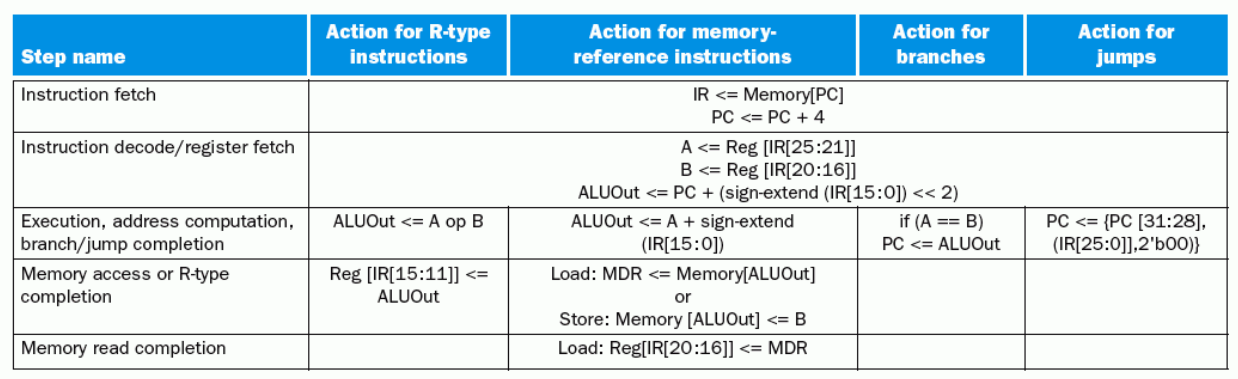
\includegraphics[scale=0.3]{mc2.png}
	    	\caption{Resumo de Operações}
	    	\label{Resumo de Operações}
		\end{figure}


		\subsection{Unidade de Controlo}

		No datapath Syngle-Cycle, no qual as instruções se executam num único ciclo de relógio e por isso
		a unidade de controlo é apenas responsável pela  geração de sinais que se mantêm inalterados ao
		longo da execução de uma determinada instrução,sendo a lógica de controlo é puramente combinatória.

		A unidade de controlo do datapath Multi-Cycle passa a ser uma máquina de estados, já que é necessário gerar sinais diferentes
		para as várias fases de execução das diferentes instruções suportadas pelo datapath,
		o que impossibilita a utilização de apenas lógica combinatória.

	  \subsubsection{A máquina de Estados}
		A máquina de estados da unidade de controlo do datapath contem dez estados diferentes, abaixo explicados.



		Como os dois primeiros ciclos de execução são comuns a todas as instruções, correspondem a dois estados de execução.
		O primeiro estado corresponde à primeira fase de processamento(\textit{Instruction Fetch}), o segundo como seria expectável é a fase de \textit{Instruction Decode}, este estado tem cinco destinos diferentes.
		Os possiveis estados de destino serão:
		\begin{itemize}
			\item SLTI-> encaminha para os estados responsáveis pela execução destas operações;
			\item ADDI,SW,LW;
			\item Instruções do tipo R;
			\item beq;
			\item jump;
		\end{itemize}


			\subparagraph{Instruções do tipo R}
			 	Para executar as operações de tipo R são necessários dois estados adicionais, um deles para contolar a ALU para que esta desempenhe a operação designada pelas operações fornecidas, assimcomo assegurar que os dados que entram na ALU são os corretos.

				O ultimo estado  grava o valor calculado no registo de destino indicado pela instrução.

			\subparagraph{ADDI}
				A execução da instrução ADDI exige que sejam criados dois estados adicionados, sendo que o primeiro tem como função definir a operação a re alizar pela ALU e assegurar a correto encaminhamento dos operandos para a mesma.

				O último tal guarda o valor calculado pela ALU num registo.

			\subparagraph{SLTI}

				Para realizar esta operação é necessário assegurar o encaminhamento do segundo operando e garantir que ALU efetue a operação correta, o estado de escrita no registo é garantido pelo mesmo estado da instrução anterior(???).



				\begin{figure}[htp]
			    	\centering
			    	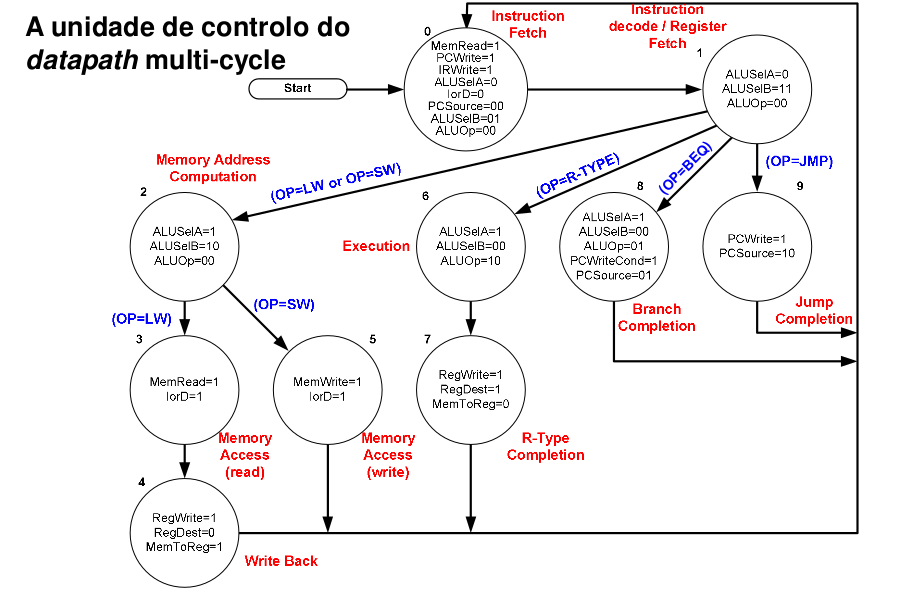
\includegraphics[scale=0.4]{FSm.png}
			    	\caption{Estados da Unidade de Controlo }
			    	\label{multy-cycle FSM}
				\end{figure}


  \section{Pipeline}

    Esta estratégia para a implementação do datapath permite aumentar o numero de instruções executadas num determinado momento para o (número de instruções*numero de fases(F) do pipeline)-1. Aprofundando, ao invés de executar uma instrução exclusiva em cinco ciclos de relógio(numero de fases do pipeline apresentado), aproveita os elementos lógicos(que se enquadram numa determinada fase de execução) que vão sendo libertadas na execução de uma primeira instrução, quando a primeira instrução liberta uma das fases uma segunda instrução entra no datapath e dá-se inicio à sua execução na fase que fora libertada anteriormente.

		\subsection{Estrutura}

			Pegando no datapath Single-Cycle, é possível dividi-lo em fases de execução.
			\begin{enumerate}
				\item Instruction Fetch;
				\item Insruction Decode;
				\item Execute;
				\item Memory Access;
				\item Write Back;
			\end{enumerate}

			\begin{figure}[htp]
					\centering
					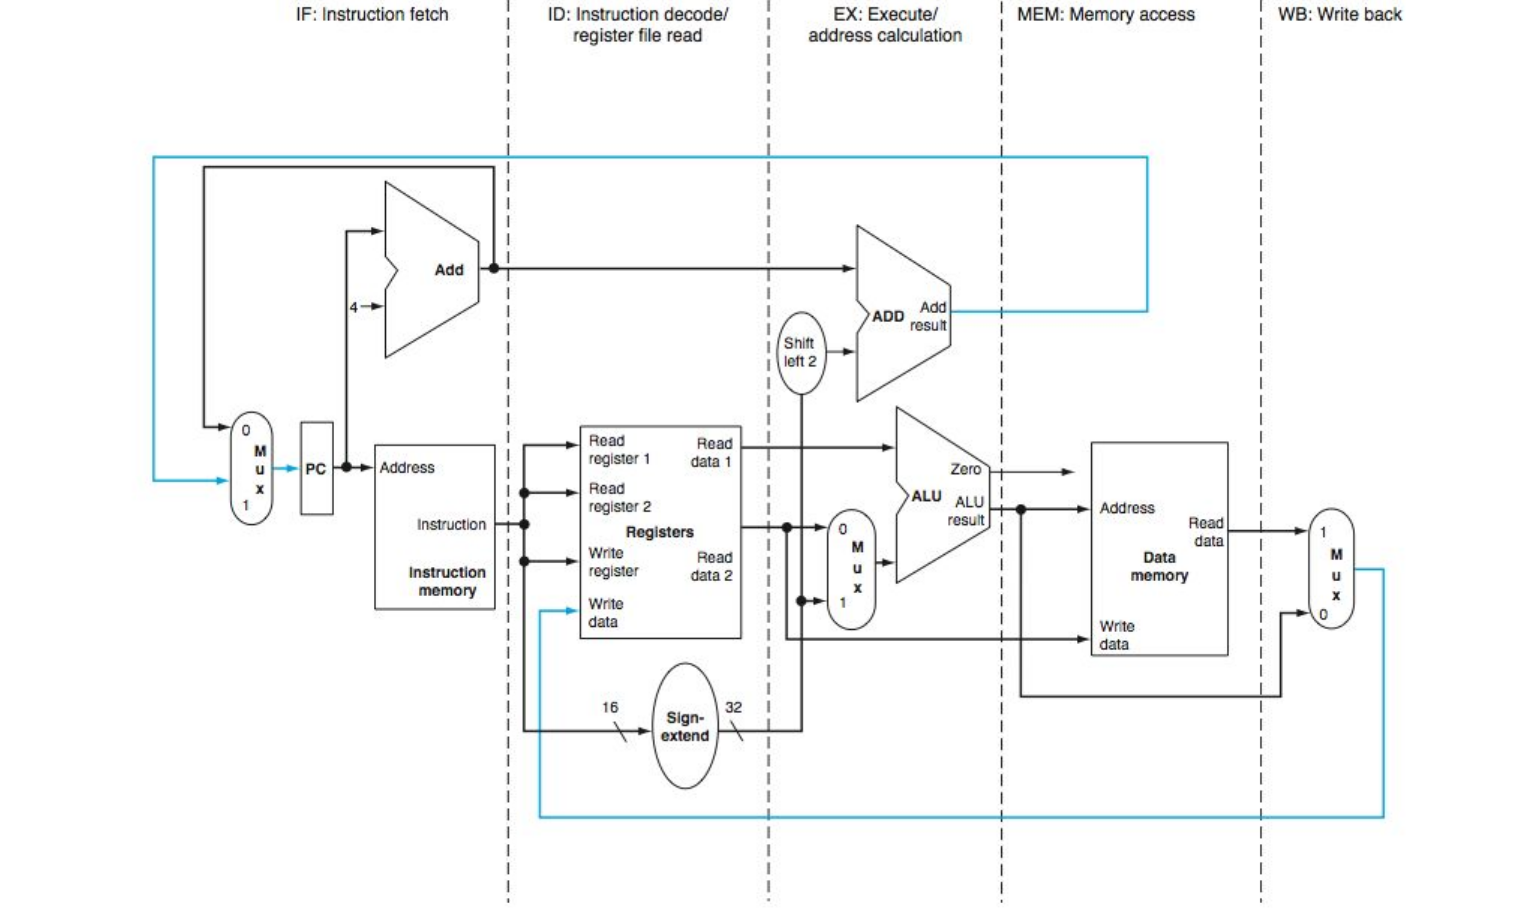
\includegraphics[scale=0.3]{pipeline3.png}
					\caption{Datapath Single-Cycle dividio nas fases de execução }
					\label{SC-division}
			\end{figure}

			Como as instruções são executadas ao longo de vários ciclos de relógio é necessário guardar os valores que vão passando de uma fase para a outra do pipeline. Para isso foram criados registos que se encontram entre as fases de processamento do pipeline.
			\begin{itemize}
				\item IF/ID;
				\item ID/EX;
				\item EXE/MEM;
				\item MEM/WB;
			\end{itemize}

			Conforme as instruções vão sendo executadas e dependendo do tipo de instruções, os dados necessários são retransmitidos de fase para fase, ou seja, transitam de registo para registo.

			Assim obtemos um datapath Pipelined muito simplificado, no final da secção de hazards é possível encontrar um datapath mais avançado que suporta a resolução de hazards.

			Pode-se concluir que os elementos lógicos existentes em cada fase só podem ser usados uma vez por ciclo de relógio.

			\begin{figure}[htp]
					\centering
					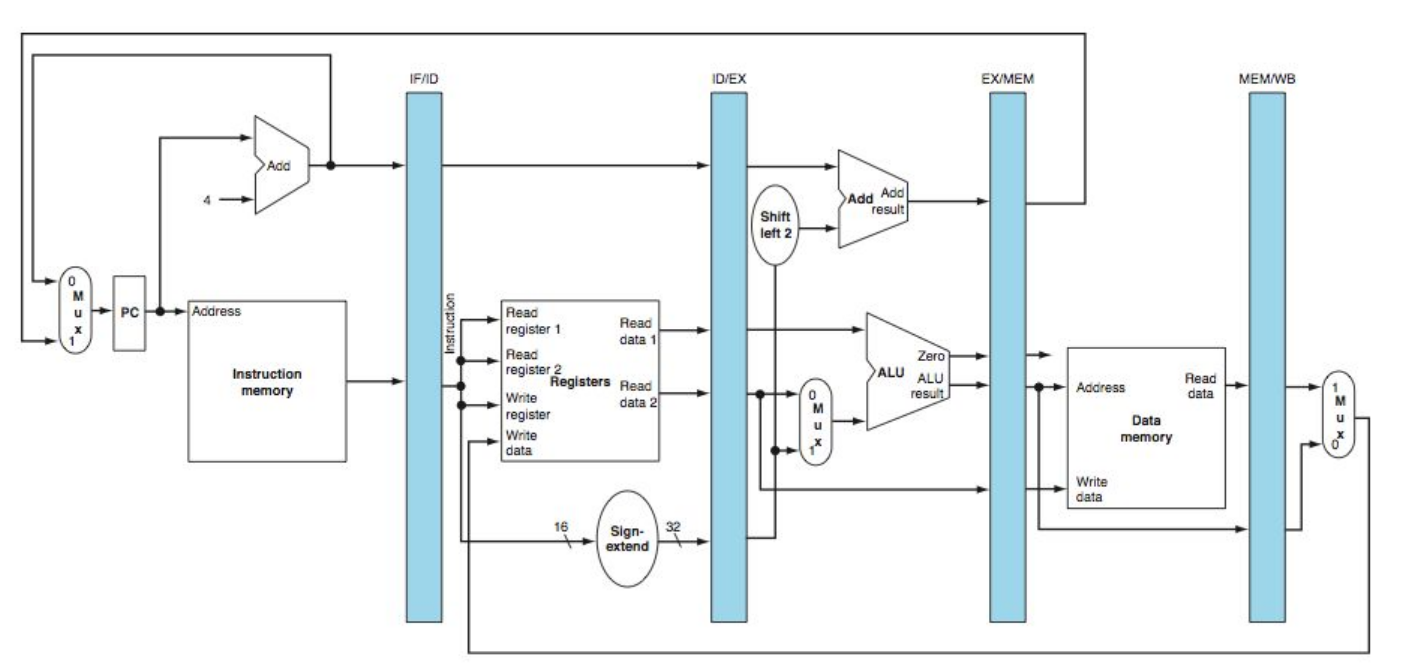
\includegraphics[scale=0.3]{pipeline4.png}
					\caption{Datapath Pipelined simples}
					\label{simple-pipelined}
			\end{figure}


		\subsection{Unidade de Controlo}

		A unidade do datapath pipelined é semelhante à do datapath Single-Cycle. É uma unidade combinatória que gera os sinais de controlo em função da instrução a executar.
		os sinais de controlo avançam ao longo das fases do pipeline.

		Os sinais de controlo utilizados são em tudo semelhantes aos usados no datapath ao single cycle.

		É possível dividir as linhas de controlo pelas várias fases de processamento.

		\paragraph{Instructon Fetch} Os sinais de controlo utilizados para ler a memória de instruções e o PC estão sempre assegurado, não é necessário nenhum sinal de controlo adicional.

		\paragraph{Instruction Decode/register file read} Tal como na fase anterior não é necessário nenhum sinal de controlo especifico para esta fase.

		\paragraph{Execution} Nesta fase já são necessários sinais de controlo especificos:
		\begin{itemize}
			\item RegDst;
			\item ALUOp;
			\item ALUsrc;
		\end{itemize}

		Estes sinais tal como no datapath Single Cycle permitem selecionar o registo de destino, a operação a executar na alu e direcionar,conforme a instrução a ser executada, os sinais provenientes do signal extender ou da saida ReadData2.

		\paragraph{Memory Access} Os sinais de controlo nesta fase são os sinais de Branch, MemRead e MemWrite. Sinais que variam conforme a instrução a executar.

		\paragraph{Write Back} As linhas de controlo existentes nesta fase são o MemtoReg e o RegWrite. O primeiro decide entre mandar o resultado proveniente da ALU ou  o valor de memória para um Registo, já o segundo escreve o valor escolhido anteriormente.

		\begin{figure}[htp]
				\centering
				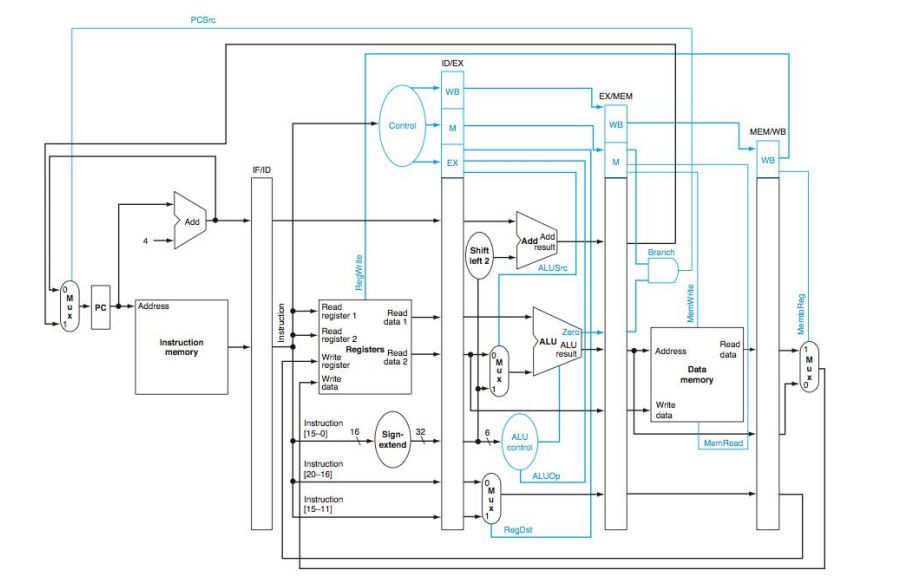
\includegraphics[scale=0.4]{pipeline5.png}
				\caption{Datapath Pipelined com sinais de controlo}
				\label{simple-pipelined-ctl}
		\end{figure}



		\subsection{Hazards}
			No seguimento da execução de várias instruções podem haver problemas tais como acessos simultâneos à memória, ou sobreposição de registos, por exemplo quando se efetua o instruion fetch e em simultâneo outra fase mais adiantada de execução faz um acesso à memória.

			Outro exemplo

			\begin{lstlisting}

			 add $s0,$t0,$t1$
			 sub $t2,$s0,$t3
			 lw $t4,0($t2)

			\end{lstlisting}

			Neste exemplo vemos que o registo s0  é usado pela instrução seguinte, o problema surge porque a instrução add não é concluida a tempo de forncer o resultado para correto. para que a operção seguinte(sub).

			Aos problemas que surgem durante a execução das intruçoes ao longo dos vários ciclos de relógio no pipeline dá-se o nome de Hazards.

			Existem três tipos de Hazards:

			\begin{itemize}
				\item Hazards Estruturais;
				\item Hazards de Dados;
				\item Hazards de Controlo;
			\end{itemize}

		\subsubsection{Hazards Estruturais}

			Este tipode hazards ocorre quando o Hardware não suporta a execução de uma combinação de instruções num único ciclo de relógio, ou seja, quando uma instrução tem que aceder ao mesmo hardware no mesmo ciclo de relógio. Surgem associados a acessos simultâneos à memória, problema que é resolvido usando duas memŕorias no datapath, uma para os dados e outra para o programa.

			\begin{figure}[htp]
					\centering
					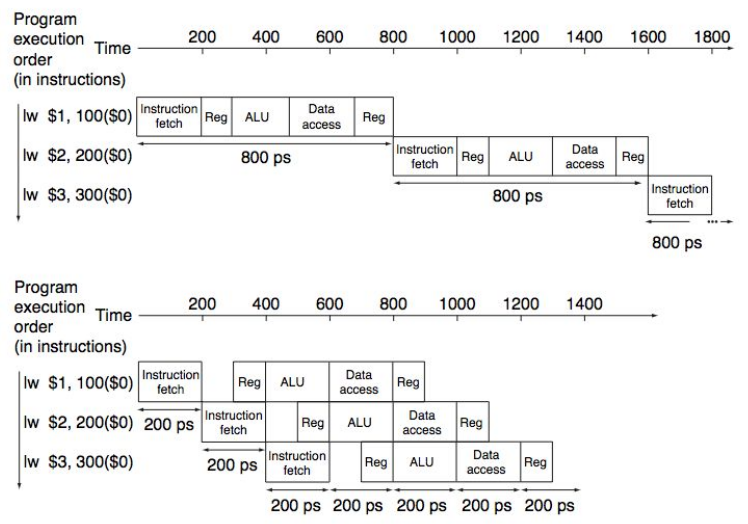
\includegraphics[scale=0.4]{pipeline1.png}
					\caption{Execução de instruções: Outros vs Pipeline}
					\label{Others vs Pipeline}
			\end{figure}

	  \subsubsection{Hazard de Controlo}

			Este tipo de hazards ocorre quando é necessário parar a execução das instruções no pipeline.
			Quando é executado um instruction fetch para uma instrução, mas existe uma instrução,mais avançada no pipeline, que pode pudar o curso de execução do programa.
			Conclui-se que estes hazards surgem associados às instruções que envolvem branches e jumps.

			Existem três maneiras de lidar com Hazards de Controlo:

			\begin{itemize}
				\item Stalling;
				\item Previsão;
				\item Delayed Branch;
			\end{itemize}

			\paragraph{Stalling}

				O Stalling consiste em atrasar a entrada de uma nova instrução no pipeline até que se saiba o resultado da instrução anterior.
        \begin{figure}[htp]
            \centering
            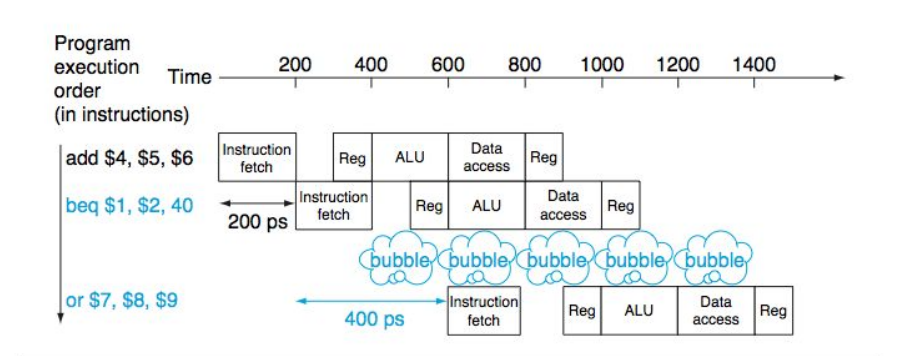
\includegraphics[scale=0.4]{pipeline2.png}
            \caption{Stalling em todos os Branches}
            \label{Stalling}
        \end{figure}
				Assim que é detetado um branch a instrução que se encontra a seguir é substituida por um nop(por exemplo um sll 0,0,0)

				Esta alternativa é eficaz mas não eficiente, uma vez que implica a paragem do datapath. Revela-se,assim, demasiado lenta para ser adotada, subretudo em pipelines com várias fases.
				Torna-se imperativo encontrar uma outra solução.

			\paragraph{Previsão}

				Nesta aboragem quando os branches são detetados são considerados como \textit{not taken}, isto é, o resultado do branch é false.

				Caso a previsão esteja errada a unidade de contolo do pipeline força o datapath a reiniciar a execução da instrução, substitui a instrução a seguir ao branch por uma NOP e continua o Instruction Fetch da operação correcta.

				Quando se usam previsores estáticos(previsores taken, ou not-taken) o resultado da previsão não depende do resultado das instruções.

				Nesta sebenta apenas iremos abordar a previsão estática. É possível fazer previsões mais acertadas usando previsores dinâmicos para que, ao longo da execução as previsões se alterem mediante os resultandos que vão sendo obtidos.Este tipo de previsores permite optimizar a previsão por forma a acertar em 90 das situações de branch.

				Comparado com o stalling a previsão permite optimizar o pipeline, msmo assim quando a previsão está errada vão-e perder ciclos de processamento.


      \paragraph{Branch Delay Slot}

				O Branch Delay Slot consiste em executar a instrução imdeiatamente a seguir ao branch, quer este seja taken or not taken.

        Esta técnica é aplicada ao nivel do software, neste caso o compilador que organiza as as instruções por forma a reposicionar o branch para aumentar a eficiência. Esta troca só é feita quando não existem implicações na execução do programa. Quando o compiilador não consegue aplicar estas mudanças é introduzida uma NOP.


		\subsubsection{Hazards de Dados}

		Quando há dependência do resultado de uma instrução com o operando de uma instrução que se encontra mais atrasada no pipeline estamos perante um hazard de dados.


		Se o resultado que vai ser necessário pela instrução atrasada ainda não tiver sido armazenado em memória não se pode prosseguir a execução, já que vai ser usado como operando um valor destualizado e, por isso ,errado.

		Podemos concluir que estes hazards ocorrem quando uma instrução  opera sobre dados, dados estes que estão a ser manipulados por instruções mais à frente no pipeline.

		Há duas soluções para este problema :
		 \begin{itemize}
			 \item Forwarding
			 \item Stalling
	 \end{itemize}


	 \paragraph{Forwarding}

	 Ao observar a execução das várias instruções suportadas pelo pipeline é possível concluir que não é preciso esperar cinco fases para obter o resultado válido de uma instrução, muitos hazards podem ser resolvidos antecipando a aquisição dos resultados necessários. Por exemplo, as instruções do tipo R calculam o resultado na terceira fase de execução(EX), podendo o resultado ser disponibilizado para a instrução seguinte. A este processo dá-se o nome de Forwarding, ou Bypassing

	 Este método só pode ser aplicado se houver uma relação de causalidade entre as operações, isto é, só se pode fazer forwarding de dados para uma fase de dados subsequente, ou seja, que não tenha ocorrido.Quando não se verifica a causalidade temos que recorrer a soluções como o stalling.


	 Exemplos...

	 Por forma a resolver um hazard de de dados é ncessário que primeiro, sejam detetados os Hazards e segundo, é preciso garantir que se faz encaminhamento do valor ou valores pelas diferentes fases de execução do pipeline que se encontram mais avançadas.
	 A maior parte dos hazards são resolvidos encaminhando os valores que se encontram em fases mais avançadas do pipeline para, normalmente, a fase EX, fase em que são necessários, com excepção dos \textit{branches}, os valores corretos para os registos a manipular pela ALU.


	\paragraph{Forwarding Control Unit}

   As situações de hazard que carecem de rencaminhamento(forwarding) podem ser facilmente identificadas:
	 \begin{enumerate}
		 \item Instrução na fase MEM cujo destino é o registo de uma instrução que se encontra na fase de EX.
 		\item Uma instrução que se encontra em WB cujo registo de destino seja um registo de uma instrução na fase de EX
	 \end{enumerate}


	\subparagraph{1}
		De forma simplificada temos que:

		\textbf{EX/MEM.RDD} == \textbf{ID/EX.RS} ou

		\textbf{EX/MEM.RDD} == \textbf{ID/EX.RT}

	 Exemplificando
		\begin{lstlisting}
			MEM add $1,$2,$3
			EX sub $4,$1,$5

	  \end{lstlisting}

		\subparagraph{2}
			De forma simplificada temos que:

			\textbf{MEM/WB.RDD} == \textbf{ID/EX.RS} ou

			\textbf{MEM/WB.RDD} == \textbf{ID/EX.RT}

		 Exemplificando
			\begin{lstlisting}
				WB  add $1,$2,$3
				ME; add $6,$2,$3
				EX  sub $4,$5,$1

		  \end{lstlisting}

		Exemplo Slides(61)

		\newline

		Embora as situações acima referidas permitam fazer uma deteção de Hazards esta não é suficiente, para o ser é ncessário avaliar o valor do sinal que controla a escrita nos registos(RegDst)

		\newline
		Ficamos com:

		(\textbf{EX/MEM.RegWrite} == 1) and(\textbf{MEM/WB.RDD} == \textbf{ID/EX.RS}) ou

		(\textbf{EX/MEM.RegWrite} == 1) and ()\textbf{MEM/WB.RDD} == \textbf{ID/EX.RT})

		(\textbf{MEM/WB.RegWrite} == 1) and (\textbf{EX/MEM.RDD} == \textbf{ID/EX.RS}) ou

		(\textbf{MEM/WB.RegWrite} == 1) and (\textbf{EX/MEM.RDD} == \textbf{ID/EX.RT})




	 \paragraph{Stalling}

	 O Stalling, que já fora abordado levemente na introdução pipeline, consiste em parar a execução das instruções durante um ou mais ciclos de relógio.


	 Esta é uma alternativa que torna o cpu pouco eficiente. Atualmente ,para evitar este tipo de situação(stalling) os compiladores tentam efetuar uma reordenação de instruções sem alterar o resultado final do programa. Vejamos o seguinte exemplo:

	 \begin{lstlisting}

    lw $t0,0($t1)
		lw $t2,4(t1)
		sub $s0,$t1,$t2 #Aqui ocorre stalling causado por um Hazzard de dados
		sw  $t0,4(t1)
 		#efetuando uma troca ficamos com:
		lw $t0,0($t1)
		lw $t2,4(t1)
		sw  $t0,4(t1)
		sub $s0,$t1,$t2 #efetivamente a troca da instrução de sub com a sw não tem efeito no resultado final do programa
	 \end{lstlisting}





























 		\printindex
\end{document}
